\documentclass[a4paper,12pt,french]{article}

\usepackage[cours]{../../../Style}

%\selectcolormodel{cmyk}

%\usepackage{wrapfig}

% Début du document
%%%%%%%%%%%%%%%%%%%
\begin{document}

\title{Dérivation}
\maketitle

\begin{programme}
\item Point de vue local:
\begin{itemize}
\item Sécantes à une courbe passant par un point donné, taux de variation en un point
\item Tangente à une courbe en un point, définie comme position limite des sécantes
\item Nombre dérivé en un point défini comme limite du taux de variation
\item Equation réduite de la tangente en un point.
\end{itemize}
\item Point de vue global
\begin{itemize}
\item Fonction dérivée
\item Dérivées de $x \mapsto x^2$, $x \mapsto x^3$, de combinaisons linéaires, de polynômes de degré $\leq 3$
\item Sens de variation d'une fonction, lien avec le signe de la dérivée
\item Tableau de variations, extremums
\end{itemize}
\item Capacités
\begin{itemize}
\item Interprétation du nombre dérivé comme coeff directeur de la tangente
\item Construire la tangente à une courbe en un point
\item Déterminer l'équation réduite de la tangente à une courbe en un point
\item Calculer la dérivée d'un polynome de degré $\leq 3$
\item Déterminer le sens de variation et les extremums d'une fonction polynome de degré $\leq 3$
\end{itemize}
\end{programme}

\section{Point de vue local}

\subsection{Tangentes}

\compo
{
\begin{center}
\begin{tikzpicture}[scale=\echellepgf]
\begin{axis}[
styleglobal,
width=0.8*\echellepgfinv*\linewidth,
xmin=-1, xmax=4,
ymin=-1, ymax=4,
xtick distance=1,
ytick distance=1,
ticks=none,
declare function={f(\x)=e^(0.75*(\x-1)-0.5);}
]
\addplot[styleplot]{f(x)} node [pos=0.75,below right] {$\mathscr C_f$};
\node[stylepoint,fill=blue] (A) at (0.5,{f(0.5)}) {};
\node[stylepoint,fill=blue] (B) at (2.5,{f(2.5)}) {};
\draw[color=blue,dashed,very thick] (0.5, 0) -- (A) node [pos=0,below] {$a$};% -- (0,{f(0.5)}) node [pos=1,left] {$f(x)$};
\draw[color=blue,dashed,very thick] (2.5, 0) -- (B) node [pos=0,below] {$a+h$};% -- (0,{f(1.2)}) node [pos=1,left] {$f(y)$};
\draw[line width=1.3pt,shorten <= -20cm,shorten >= -20cm,densely dotted] (A) -- (B);
\end{axis}
\end{tikzpicture}
\end{center}
}
{
\begin{center}
\begin{tikzpicture}[scale=\echellepgf]
\begin{axis}[
styleglobal,
width=0.8*\echellepgfinv*\linewidth,
xmin=-1, xmax=4,
ymin=-1, ymax=4,
xtick distance=1,
ytick distance=1,
ticks=none,
declare function={f(\x)=e^(0.75*(\x-1)-0.5);}
]
\addplot[styleplot]{f(x)} node [pos=0.75,below right] {$\mathscr C_f$};
\node[stylepoint,fill=blue] (A) at (0.5,{f(0.5)}) {};
\node[stylepoint,fill=blue,inner sep=1.3pt] (B) at (2.5,{f(2.5)}) {};
\node[stylepoint,fill=blue,inner sep=1.5pt] (C) at (1.5,{f(1.5)}) {};
\node[stylepoint,fill=blue,inner sep=1.7pt] (D) at (0.75,{f(0.75)}) {};
\node[stylepoint,fill=blue,inner sep=1.9pt] (E) at (0.625,{f(0.625)}) {};
\draw[color=blue,dashed,thick] (0.5, 0) -- (A) node [pos=0,below] {$a$};% -- (0,{f(0.5)}) node [pos=1,left] {$f(x)$};
\draw[color=blue,dashed,thick] (2.5, 0) -- (B) node [pos=0,below] {$a+h$};% -- (0,{f(1.2)}) node [pos=1,left] {$f(y)$};
\draw[color=blue,dashed,thick] (1.5, 0) -- (C);
\draw[color=blue,dashed,thick] (0.75, 0) -- (D);
\draw[color=blue,dashed,thick] (0.625, 0) -- (E);
\draw[thick,shorten <= -20cm,shorten >= -20cm,densely dotted] (A) -- (B);
\draw[thick,shorten <= -20cm,shorten >= -20cm,densely dotted] (A) -- (C);
\draw[thick,shorten <= -20cm,shorten >= -20cm,densely dotted] (A) -- (D);
\draw[line width=1.3pt,shorten <= -20cm,shorten >= -20cm,densely dotted] (A) -- (E);
\addplot[styleplot,color=Crimson,ultra thick]{0.75*e^(0.75*(-0.5)-0.5)*(x-0.5)+f(0.5)};
\end{axis}
\end{tikzpicture}
\end{center}
}

\begin{defin}
Une fonction affine est une fonction définie sur $\R$ par $f(x)=ax+b$ où $a$ et $b$ désignent deux nombres réels donnés.
\end{defin}

\begin{exs}
$f:x \mapsto 3x+1 \ , \ g:x \mapsto \frac x 3 -2$ et $h:x \mapsto 0,1x-7,2$ sont des fonctions affines.
\end{exs}

\begin{casparts}\saut
\begin{itemize}
\item $x \mapsto ax$ (ici, $b=0$) est une fonction affine particulière appelée \emph{fonction linéaire}.
\item $x \mapsto b$ (ici, $a=0$) est une fonction affine particulière appelée \emph{fonction constante}.
\end{itemize}
\end{casparts}

\rem{Fiche tableau: reconnaissance a et b}

\section{Représentation graphique}

\begin{propr} 
Dans un repère, la représentation graphique d'une fonction affine est une \emph{droite} qui coupe l'axe des ordonnées.
\end{propr}

\begin{enonce}{Vocabulaire}
Dans un repère, soit $d$ la droite représentant une fonction affine $f:x \mapsto ax+b$. On dit que:
\begin{itemize}
\item $a$ est le \textbf{coefficient directeur} de $d$.
\item $b$ est \textbf{l'ordonnée à l'origine} de $d$.
\item $y=ax+b$ est l'équation réduite de $d$.
\end{itemize}
\end{enonce}

\begin{prop}
Lorsque $a$ s'exprime sous forme d'une fraction, on a en fait: $$a=\frac{ \text{déplacement vertical} } {\text{déplacement horizontal}}$$
\end{prop}

\begin{exs} \saut
Construisons les droites $d_1$ et $d_2$ d'équations réduites respectives $y=2x-1$ et $y=-\frac 1 3 x+3$.
\begin{itemize}
\item Pour $d_1$: L'ordonnée à l'origine de $d_1$ est $-1$, et lorsque j'avance d'un vers la droite, je monte de deux (unités).
\item Pour $d_2$: L'ordonnée à l'origine de $d_1$ est $3$, et lorsque j'avance de trois vers la droite, je descend d'un.
\end{itemize}
\begin{centrer}
\begin{tikzpicture}[scale=\echellepgf]
\begin{axis}[
styleglobal,
width=0.9*\echellepgfinv*\linewidth,
xmin=-2, xmax=11,
ymin=-2, ymax=4,
xtick distance=1,
ytick distance=1,
minor x tick num=0,
minor y tick num=0,
]
\addplot[styleplot,domain=(-2:11)]{2*x-1} node[pos=0.33,right] {$d_1$};
\draw[->,>=latex,thick] (1,1) -- (2,1) node[midway,below] {$1$};
\draw[->,>=latex,thick] (2,1) -- (2,3) node[midway,right] {$2$};
\addplot[styleplot,densely dashed,color=blue,domain=(-2:11)]{-1/3*x+3} node[pos=0.8, above right] {$d_2$};
\draw[->,>=latex,thick,color=blue] (3,2) -- (6,2) node[midway,above] {$3$};
\draw[->,>=latex,thick,color=blue] (6,2) -- (6,1) node[midway,right] {$-1$};
\end{axis}
\end{tikzpicture}
\end{centrer}
\end{exs}

\rem{Fiches construction et détermination}

\section{Recherche algébrique de $a$ et $b$}

\begin{prop}
Soit $f:x \mapsto ax+b$ une fonction affine et $x_1$ et $x_2 \in \R$, avec $x_1 \neq x_2$. Alors $$a=\frac{f(x_2)-f(x_1)}{x_2-x_1}$$
\end{prop}

\begin{ex}
On suppose que $f(1)=1$ et $f(3)=5$.

Alors $a=\dfrac{5-1}{3-1} = \dfrac 4 2 = 2$.

On a alors $f:x \mapsto 2x+b$. On sait de plus que $f(3)=2 \times 3 +b$ et $f(3)=5$ donc:
\vspace{1mm}

\compo[0.6]
{
$$\begin{aligned} &5=2 \times 3 + b \\ \text{soit donc } & 5=6+b \\ \text{et alors } & 5-6=b \\ \text{puis } & b=-1 \end{aligned}$$

Cela donne alors $f:x \mapsto 2x-1$.
}
{
\begin{centrer}
\begin{tikzpicture}[scale=\echellepgf]
\begin{axis}[
styleglobal,
width=0.9*\echellepgfinv*\linewidth,
xmin=-2, xmax=6,
ymin=-0.5, ymax=5.5,
xtick distance=1,
ytick distance=1,
]
\addplot[styleplot,domain=(-9:9)]{2*x-1};
\node[color=black,circle,minimum size=1pt,fill,inner sep=2pt] (A) at (1,1) {};
\node[color=black,circle,minimum size=1pt,fill,inner sep=2pt] (B) at (3,5) {};
\end{axis}
\end{tikzpicture}
\end{centrer}
}
\end{ex}

\rem{Fiche détermination algébrique\\Fiche preuve (*)}

\progres

\section{Tableaux de signe}

\begin{prop}
Soit $f:x \mapsto ax+b$ une fonction affine avec $a \neq 0$. Alors $f(x)=0$ si et seulement si $ax+b=0$ ssi $ax=-b$ ssi $x=-\frac b a$. Le tableau de signes de $f$ dépend du signe de $a$:

\vspace{1mm}

\compo[0.5]
{
\begin{centrer}
Si $a>0$:

\begin{tikzpicture}
\tkzTabInit[lgt=1.4,espcl=2]{$x$ /1,$f(x)$/1}{$- \infty$, $\frac {-b} a$, $+ \infty$}
\tkzTabLine{,-,z,+,}
\end{tikzpicture}
\end{centrer}
}
{
\begin{centrer}
Si $a<0$:

\begin{tikzpicture}[]
\tkzTabInit[lgt=1.4,espcl=2]{$x$ /1,$f(x)$/1}{$- \infty$, $\frac {-b} a$, $+ \infty$}
\tkzTabLine{,+,z,-,}
\end{tikzpicture}
\end{centrer}
}
\end{prop}

\begin{methode}
Grâce à la règle des signes, on peut alors dresser le tableau de signes de fonctions s'écrivant comme des produits et quotients de fonctions affines.
\end{methode}

\begin{ex}
Soit $f:x \mapsto (x+2)(4-5x)$. En décomposant $f$, on obtient alors le tableau suivant:
\begin{center}
\begin{tikzpicture}
\tkzTabInit{$x$ /1, $x+2$/1, $4-5x$/1,$f(x)$/1}{$- \infty$, $-2$, $\frac 4 5$, $+ \infty$}

\tkzTabLine{,-,z,+,t,+}
\tkzTabLine{,+,t,+,z,-}
\tkzTabLine{,-,z,+,z,-}

\end{tikzpicture}
\end{center}
On peut alors déduire de ce tableau que l'ensemble des solutions de l'inéquation $f(x) \leq 0$ est $$S=\left] - \infty;-2\right] \cup \left[\frac 4 5;+ \infty \right[$$

Pour $g:x \mapsto \dfrac{x+2}{4-5x}$, le tableau de signes obtenu est presque identique:

\begin{center}
\begin{tikzpicture}
\tkzTabInit{$x$ /1, $x+2$/1, $4-5x$/1,$g(x)$/1}{$- \infty$, $-2$, $\frac 4 5$, $+ \infty$}

\tkzTabLine{,-,z,+,t,+}
\tkzTabLine{,+,t,+,z,-}
\tkzTabLine{,-,z,+,d,-}

\end{tikzpicture}
\end{center}
La double barre signifie "non défini", dans le sens où l'on ne peut pas diviser par 0 lorsque $x=\frac 4 5$. Ce nombre n'est pas dans l'ensemble de définition de $g$.

\end{ex}

\end{document}
